\documentclass[journal]{IEEEtran} % use the `journal` option for ITherm conference style
\IEEEoverridecommandlockouts
% The preceding line is only needed to identify funding in the first footnote. If that is unneeded, please comment it out.
\usepackage{cite}
\usepackage{amsmath,amssymb,amsfonts}
\usepackage{algorithmic}
\usepackage{graphicx}
\usepackage{textcomp}
\usepackage{xcolor}
\def\BibTeX{{\rm B\kern-.05em{\sc i\kern-.025em b}\kern-.08em
    T\kern-.1667em\lower.7ex\hbox{E}\kern-.125emX}}
\begin{document}

\title{Hiding Sensitive Information in Desensitized Voice Sequences*\\
% delete or comment-out the following line before submission
{\footnotesize \textsuperscript{*}Note: Sub-titles are not captured in Xplore and should not be used}
\thanks{Identify applicable funding agency here. If none, delete this.}
}

\author{%%%% author names
    \IEEEauthorblockN{1\textsuperscript{st} Given Name Surname}% first author
    , \IEEEauthorblockN{2\textsuperscript{nd} Given Name Surname}% delete this line if not needed
    , \IEEEauthorblockN{3\textsuperscript{rd} Given Name Surname}% delete this line if not needed
    % duplicate the line above as many times as needed to list all authors
    \\%%%% author affiliations
    \IEEEauthorblockA{\textit{dept. name of organization (of Aff.), City, Country}}\\% first affiliation
    \IEEEauthorblockA{\textit{dept. name of organization (of Aff.), City, Country if needed}}\\% delete this line if not needed
    % duplicate the line above as many times as needed to list all affiliations
    %%%% corresponding author contact details
    \IEEEauthorblockA{email address or ORCID of corresponding author(s)}
}

\maketitle

\begin{abstract}
Voice data is acquired and utilized by a variety of consumer services. During the computation of such services, raw recordings of user voices is, despite the presence of offline applications, mostly sent to web servers associated with them. This imposes a significant privacy concern regarding of the nature of raw voices, which contain voiceprint and content information that is believed to be sufficient to identify the speaker or to reveal various types of sensitive information related to the speaker. In order to mitigate such problem, Desensitization methods are employed as an intermediary between user and the cloud services. However, these methods may prove not to be secure enough if they come from third parties and arrive as black-boxes. This paper discusses and demonstrates the possibility of hiding information sufficient to recover original voice from in seemingly desensitized voices that may be used for online services with deep learning technologies, utilizing StarGAN-based voice transformation and voice-optimized audio stenography technologies.
\end{abstract}

\begin{IEEEkeywords}
    privacy, voice, desensitization, stenography
\end{IEEEkeywords}

\section{Introduction}

Voice is already an important mean of human-machine interaction since the last century. Voice recognition technologies enable human to communicate with machines with voice, one of the most straightforward and comprehensive medium of human-to-human interaction. Voiceprint extraction technologies enables computers to perform authorization solely with certain features in human voices without involving traditional password-based methods, thus avoiding problems involving them.

Number of voice recognition enabled technologies is massive. Some voice assistant apps on smartphones support voiceprint-based security measures to prevent accidental (or malicious) activation by anyone other than the owner of the smartphone, such as Siri from Apple Inc. and Xiao Ai from Xiaomi Inc.\cite{a19, a20}. Also, there are many voice-typing enabled input methods for various kinds of devices, such as iFly Input Method from iFlyTek and GBoard from Google, Inc.\cite{a21, a22}.

In recent years deep learning, and deep learning based voice analysis technologies drastically advanced to a degree that generation-oriented services produce convincing voice sequences that human can't easily distinguish with authentic speeches and discrimination-oriented services provide users with accurate results that utilize even the slightest features in voice sequences that human ears are not capable of recognizing\cite{a12}.

Technologies advanced as mentioned, and voice recognition services are able to identify a person with only a sequence of its voice. This, along with concrete research findings, warned people that voices actually contain sensitive private data that is sufficient for high accuracy identification\cite{a6, a7}. If the data is handled by a company with insufficient security infrastructure or even a malicious one, it's very likely that it will result in a privacy crisis.

If the raw recordings of user's voice, which is mentioned before to contain excessive private information, is entirely handled locally on user's device (i.e. from recording to recognizing), then the security risks would not be significant since only the unidentified results are exported or sent to remote servers.

However, these recognition services consume large amount of computational power which makes it not feasible to perform the process locally on end user's device. In order to mitigate such problem, service providers resort to processing voice data in their servers. A number of vendors claimed to process the data locally, but only a portion of it, which may not meet the security demand of some consumers. For example, Xiaomi, Inc. claimed Xiao Ai to be able to "perform most of training and evaluation locally"\cite{a20}.

\begin{figure}[htbp]
    \centerline{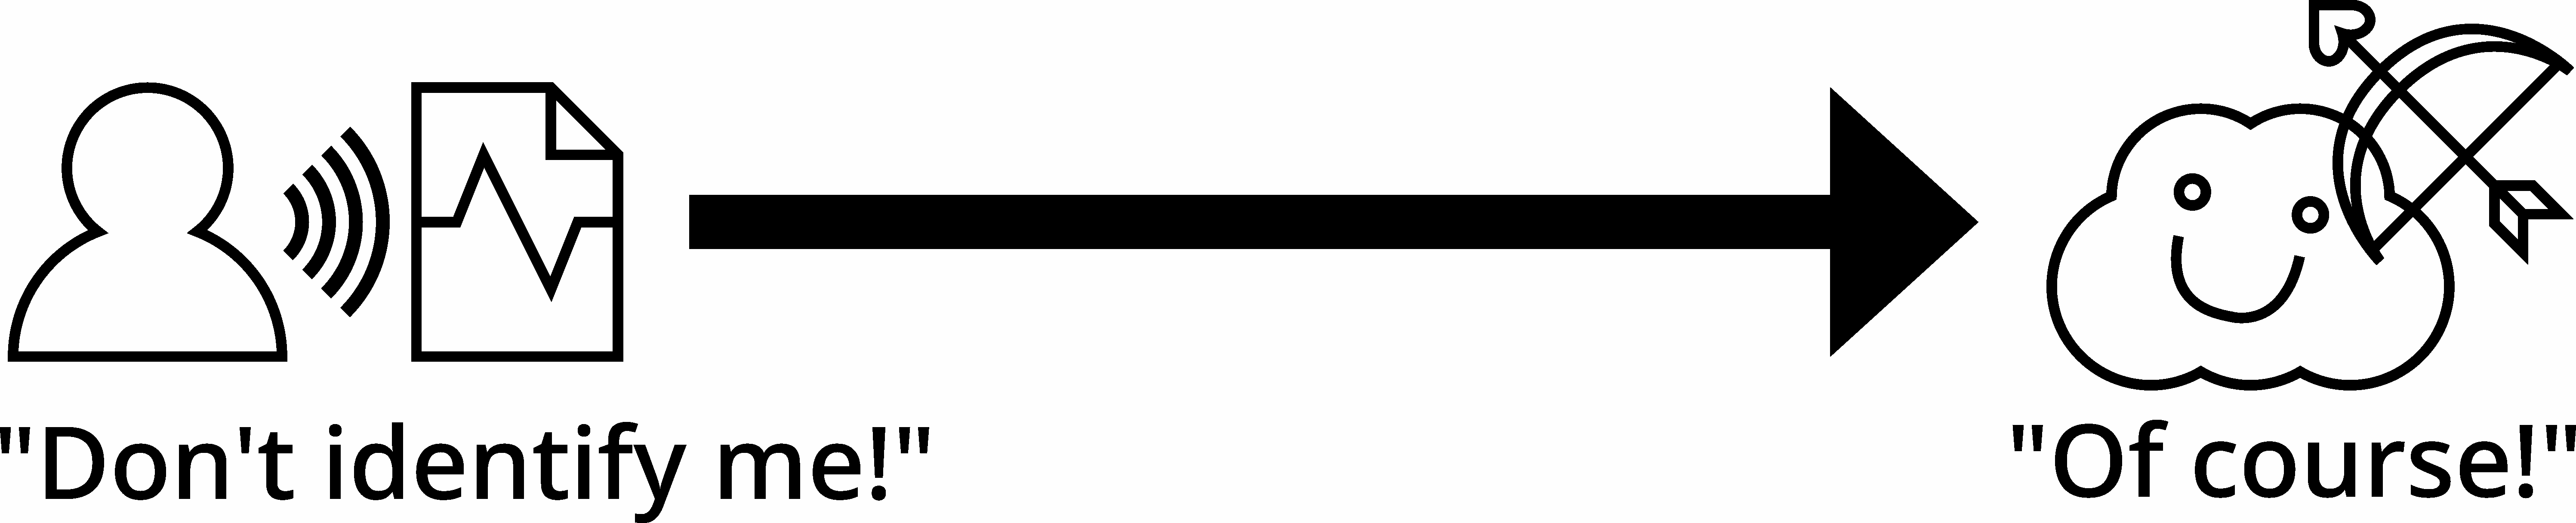
\includegraphics[width=8cm]{case1.png}}
    \caption{Case I - Idealized}
    \label{case1}
\end{figure}

\begin{figure}[htbp]
    \centerline{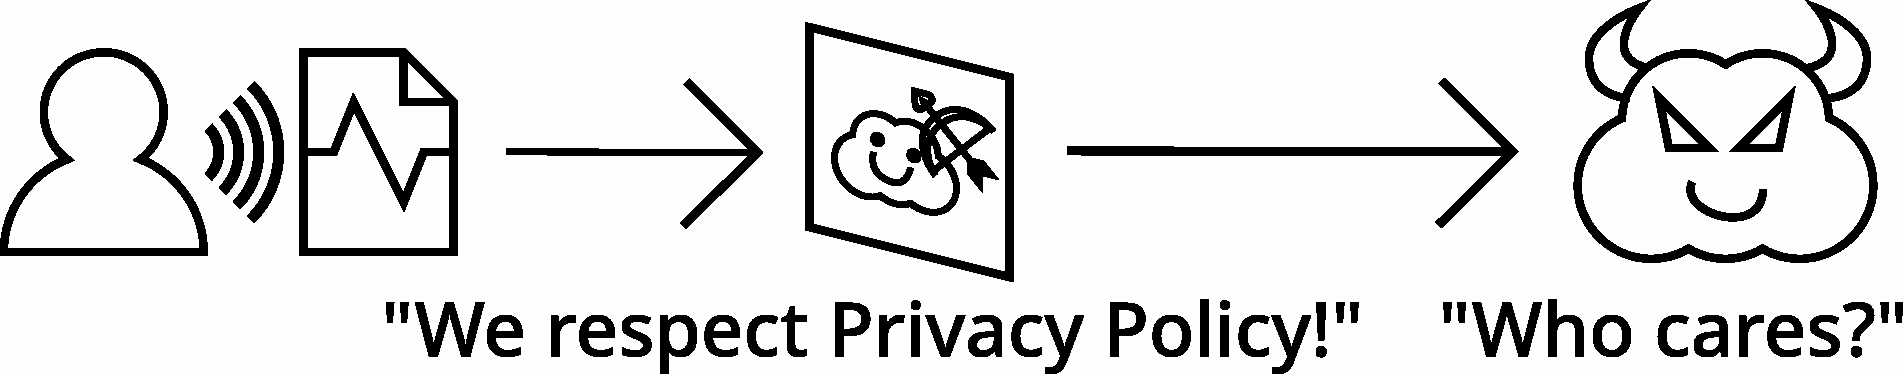
\includegraphics[width=8cm]{case2.png}}
    \caption{Case II - Reality}
    \label{case2}
\end{figure}

Ideally, an honest service provider would not use the raw recordings for anything other than the intended purpose, as depicted in Fig. 1.
However. in reality this imposes a serious privacy concern since the raw recording from user is known to contain much more data than merely for content recognition. Such additional data may be used by malicious service providers or attackers to identify the speaker and cause a data breach incident, as depicted in Fig. 2.

\begin{figure}[htbp]
    \centerline{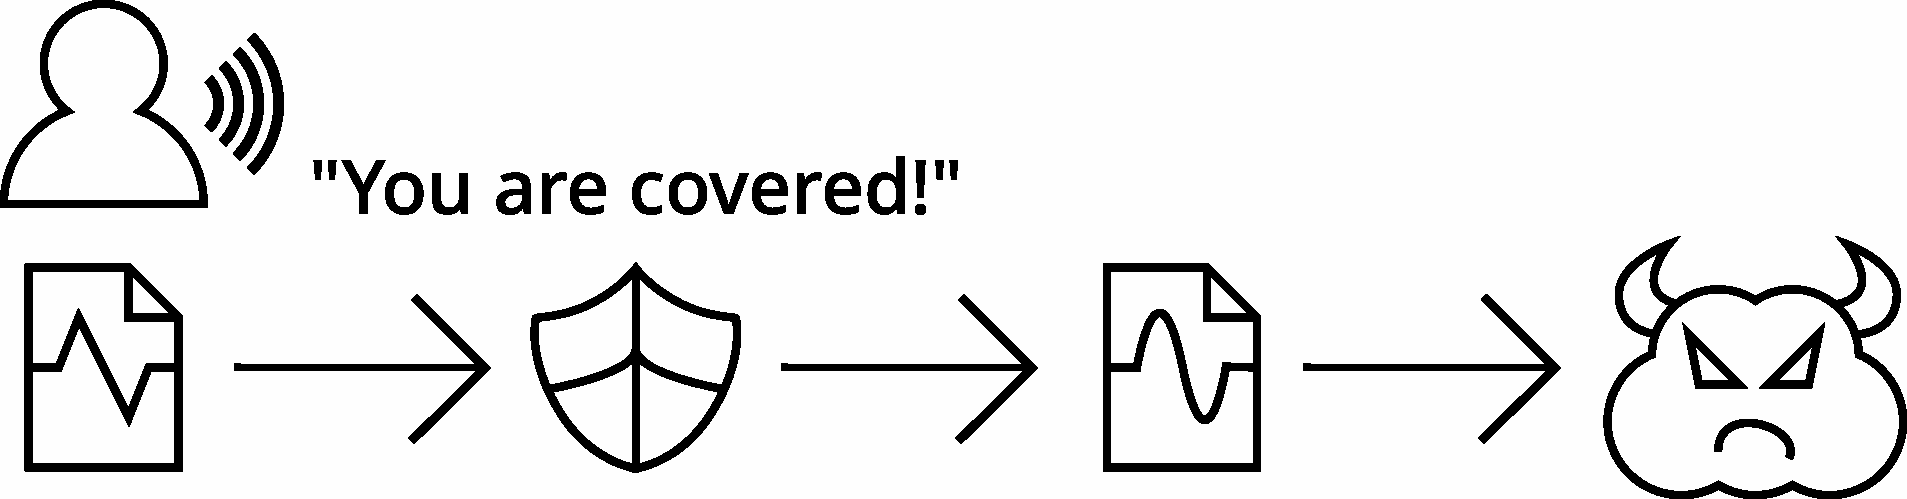
\includegraphics[width=8cm]{case3.png}}
    \caption{Case III - Mitigation}
    \label{case3}
\end{figure}

It's commonly believed that the solution to mitigate such problem is two fold: One can choose to perform all processing solely on user's device or to use certain algorithm to remove user's identity from voices before submitting to remote servers. Due to the limitations of capabilities and energy consumption, it's often likely not viable to run a large model on smartphones, laptops or other battery-powered devices. Because of that, voice desensitization algorithms are being actively developed, with the common workflow depicted in Fig. 3.

Conventional voice desensitization methods are believed to focus on two radically different areas: Content and Voiceprint.

Those which focus on content desensitization employ certain methodologies to remove or replace voice segments that are detected to potentially contain sensitive information. The detection of sensitive content is often handled by one or more deep learning based classification algorithms and the content wiping is also likely to be handled by a deep learning based transformation algorithm. 

There are publicly available APIs\cite{a13} and dedicated softwares for this purpose\cite{a14}. As a safe method or the last resort, some may employ manual audio editing to achieve this goal, and there exists a number of softwares sufficient for this use case\cite{a15}.

Other methods may apply obfuscation and distortion on entire voice sequences to decrease the possibility of associating certain features in voices with corresponding speakers. Deep learning based methodologies are also employed to distort the voice features despite the presence of a variety of traditional algorithms\cite{a9, a10, a11}.

It's notable that many approaches to bring privacy to remotely handled voices combine these 2 ideas to provide better performance. There exists a number of active researches on this subject\cite{a8}.

While evaluation of sensitive content removal is straightforward since researchers are enabled to use Text-To-Speech services with voices and compare the results with sources, the analysis of voice feature is of significantly more complexity. Obfuscation algorithms designed to disable certain recognition algorithms may not disable others and it's possible those algorithms would not confuse humans if the modification is not drastic.

\begin{figure}[htbp]
    \centerline{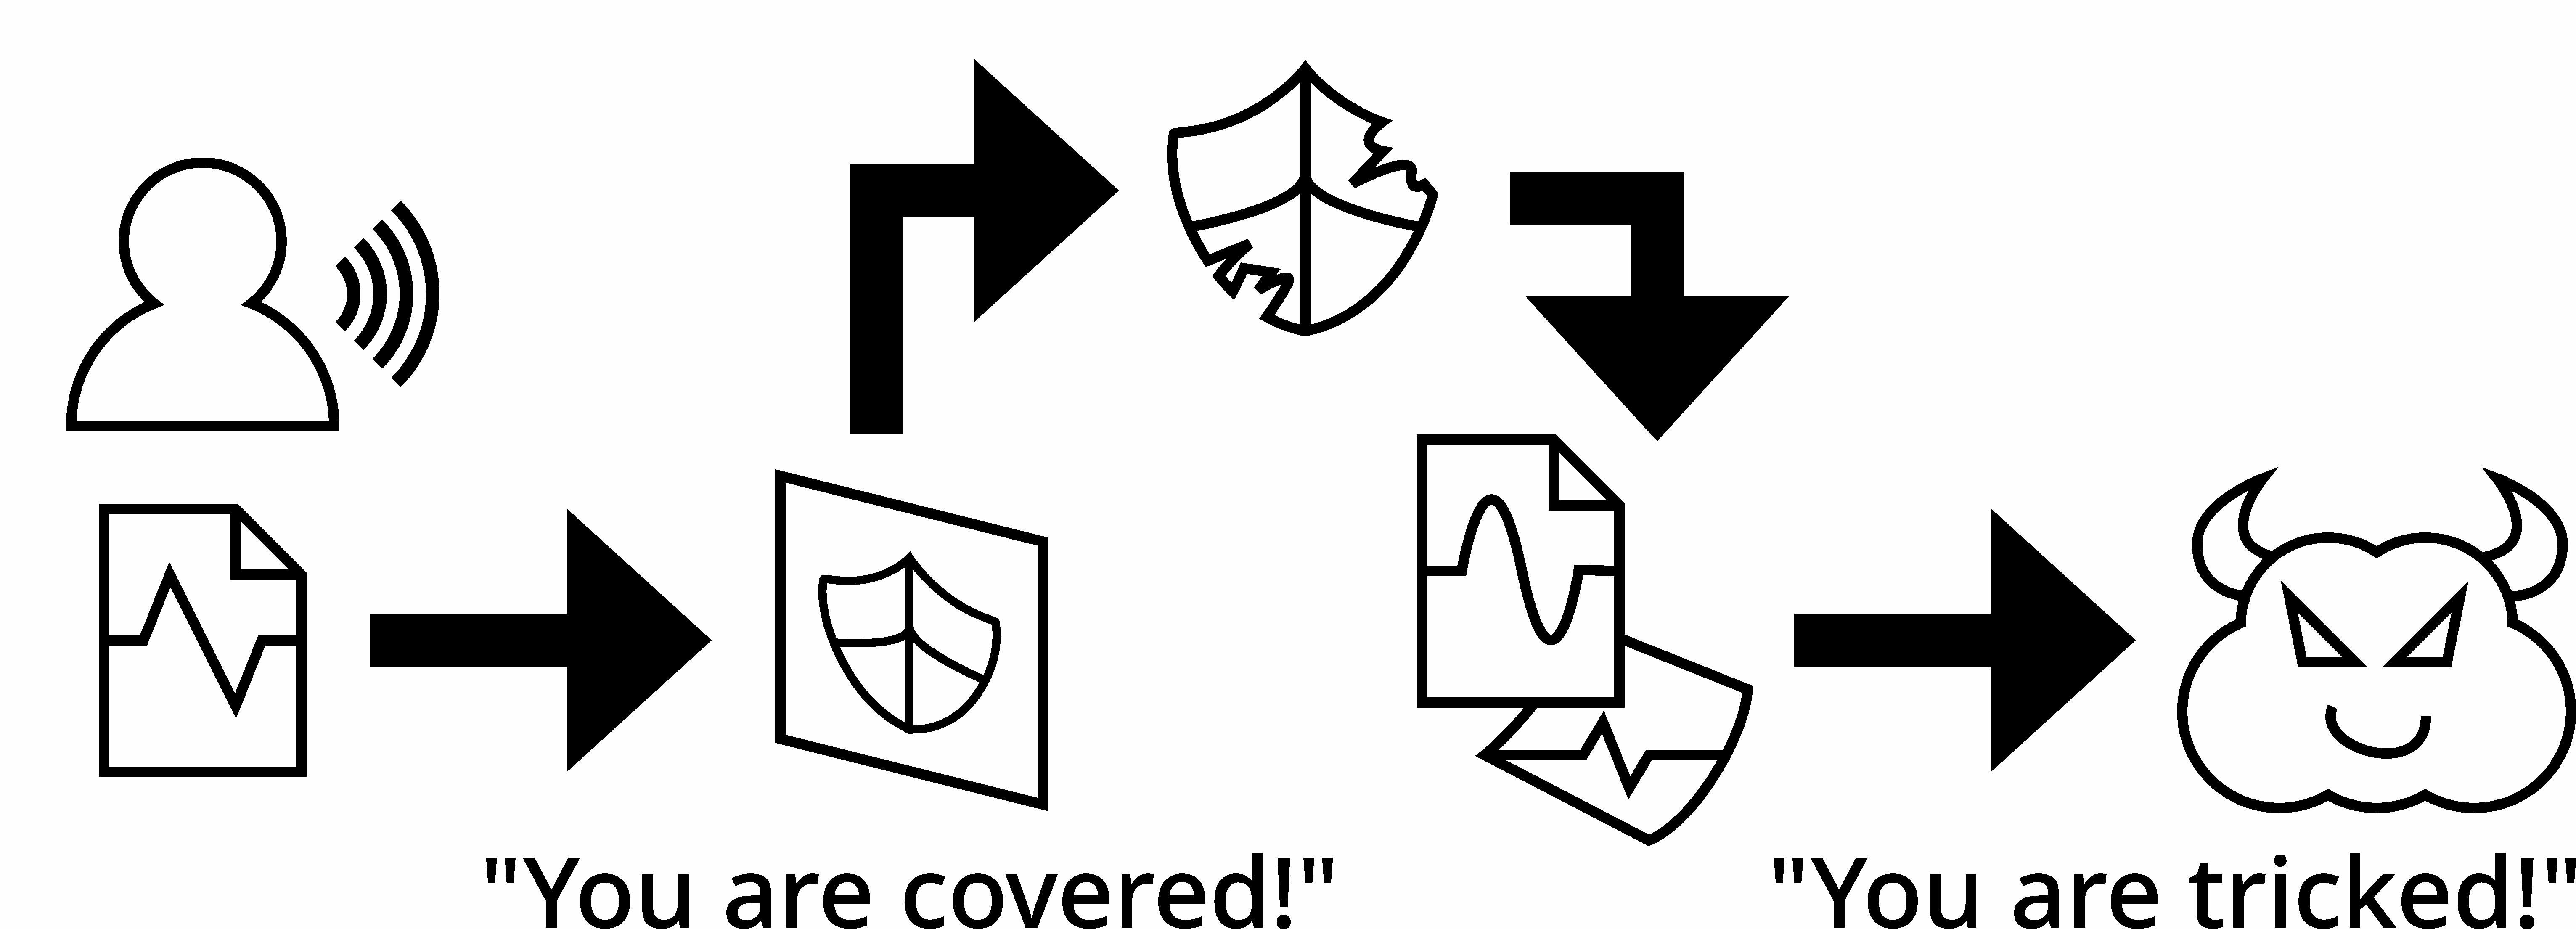
\includegraphics[width=8cm]{case4.png}}
    \caption{Case IV - Betrayal}
    \label{case4}
\end{figure}

However, the absence of sensitive data in desensitized voices can not be perfectly guaranteed. It's not only because of the incompleteness and weakness of desensitization models, but also because of the potential existence of an arbitrary algorithm that attempts to dispute this process and hide the data to recover the original voices or even the raw recording in desensitized voices by performing a slight modification, as depicted in Fig. 4. Modern deep-learning based stenography methodologies is more likely to get over a variety of stenography detection algorithms\cite{a1}, thus make the protection against such attacks more difficult.

In this paper, we demonstrate the adversarial case mentioned before with the proposal of a concrete workflow of it: a novel, adversarial utilization of various types of voice transformer frameworks that desensitize user's voices as a desensitization model, but also attempts to hide information of original voice with certain stenography technologies for another model to recovery the original one from it after the usage. The rest of the paper consists an detailed explanation of the proposed methodology, including the discussion of potential use cases and opportunities of future works.

\section{Methodology}

\begin{figure}[htbp]
    \centerline{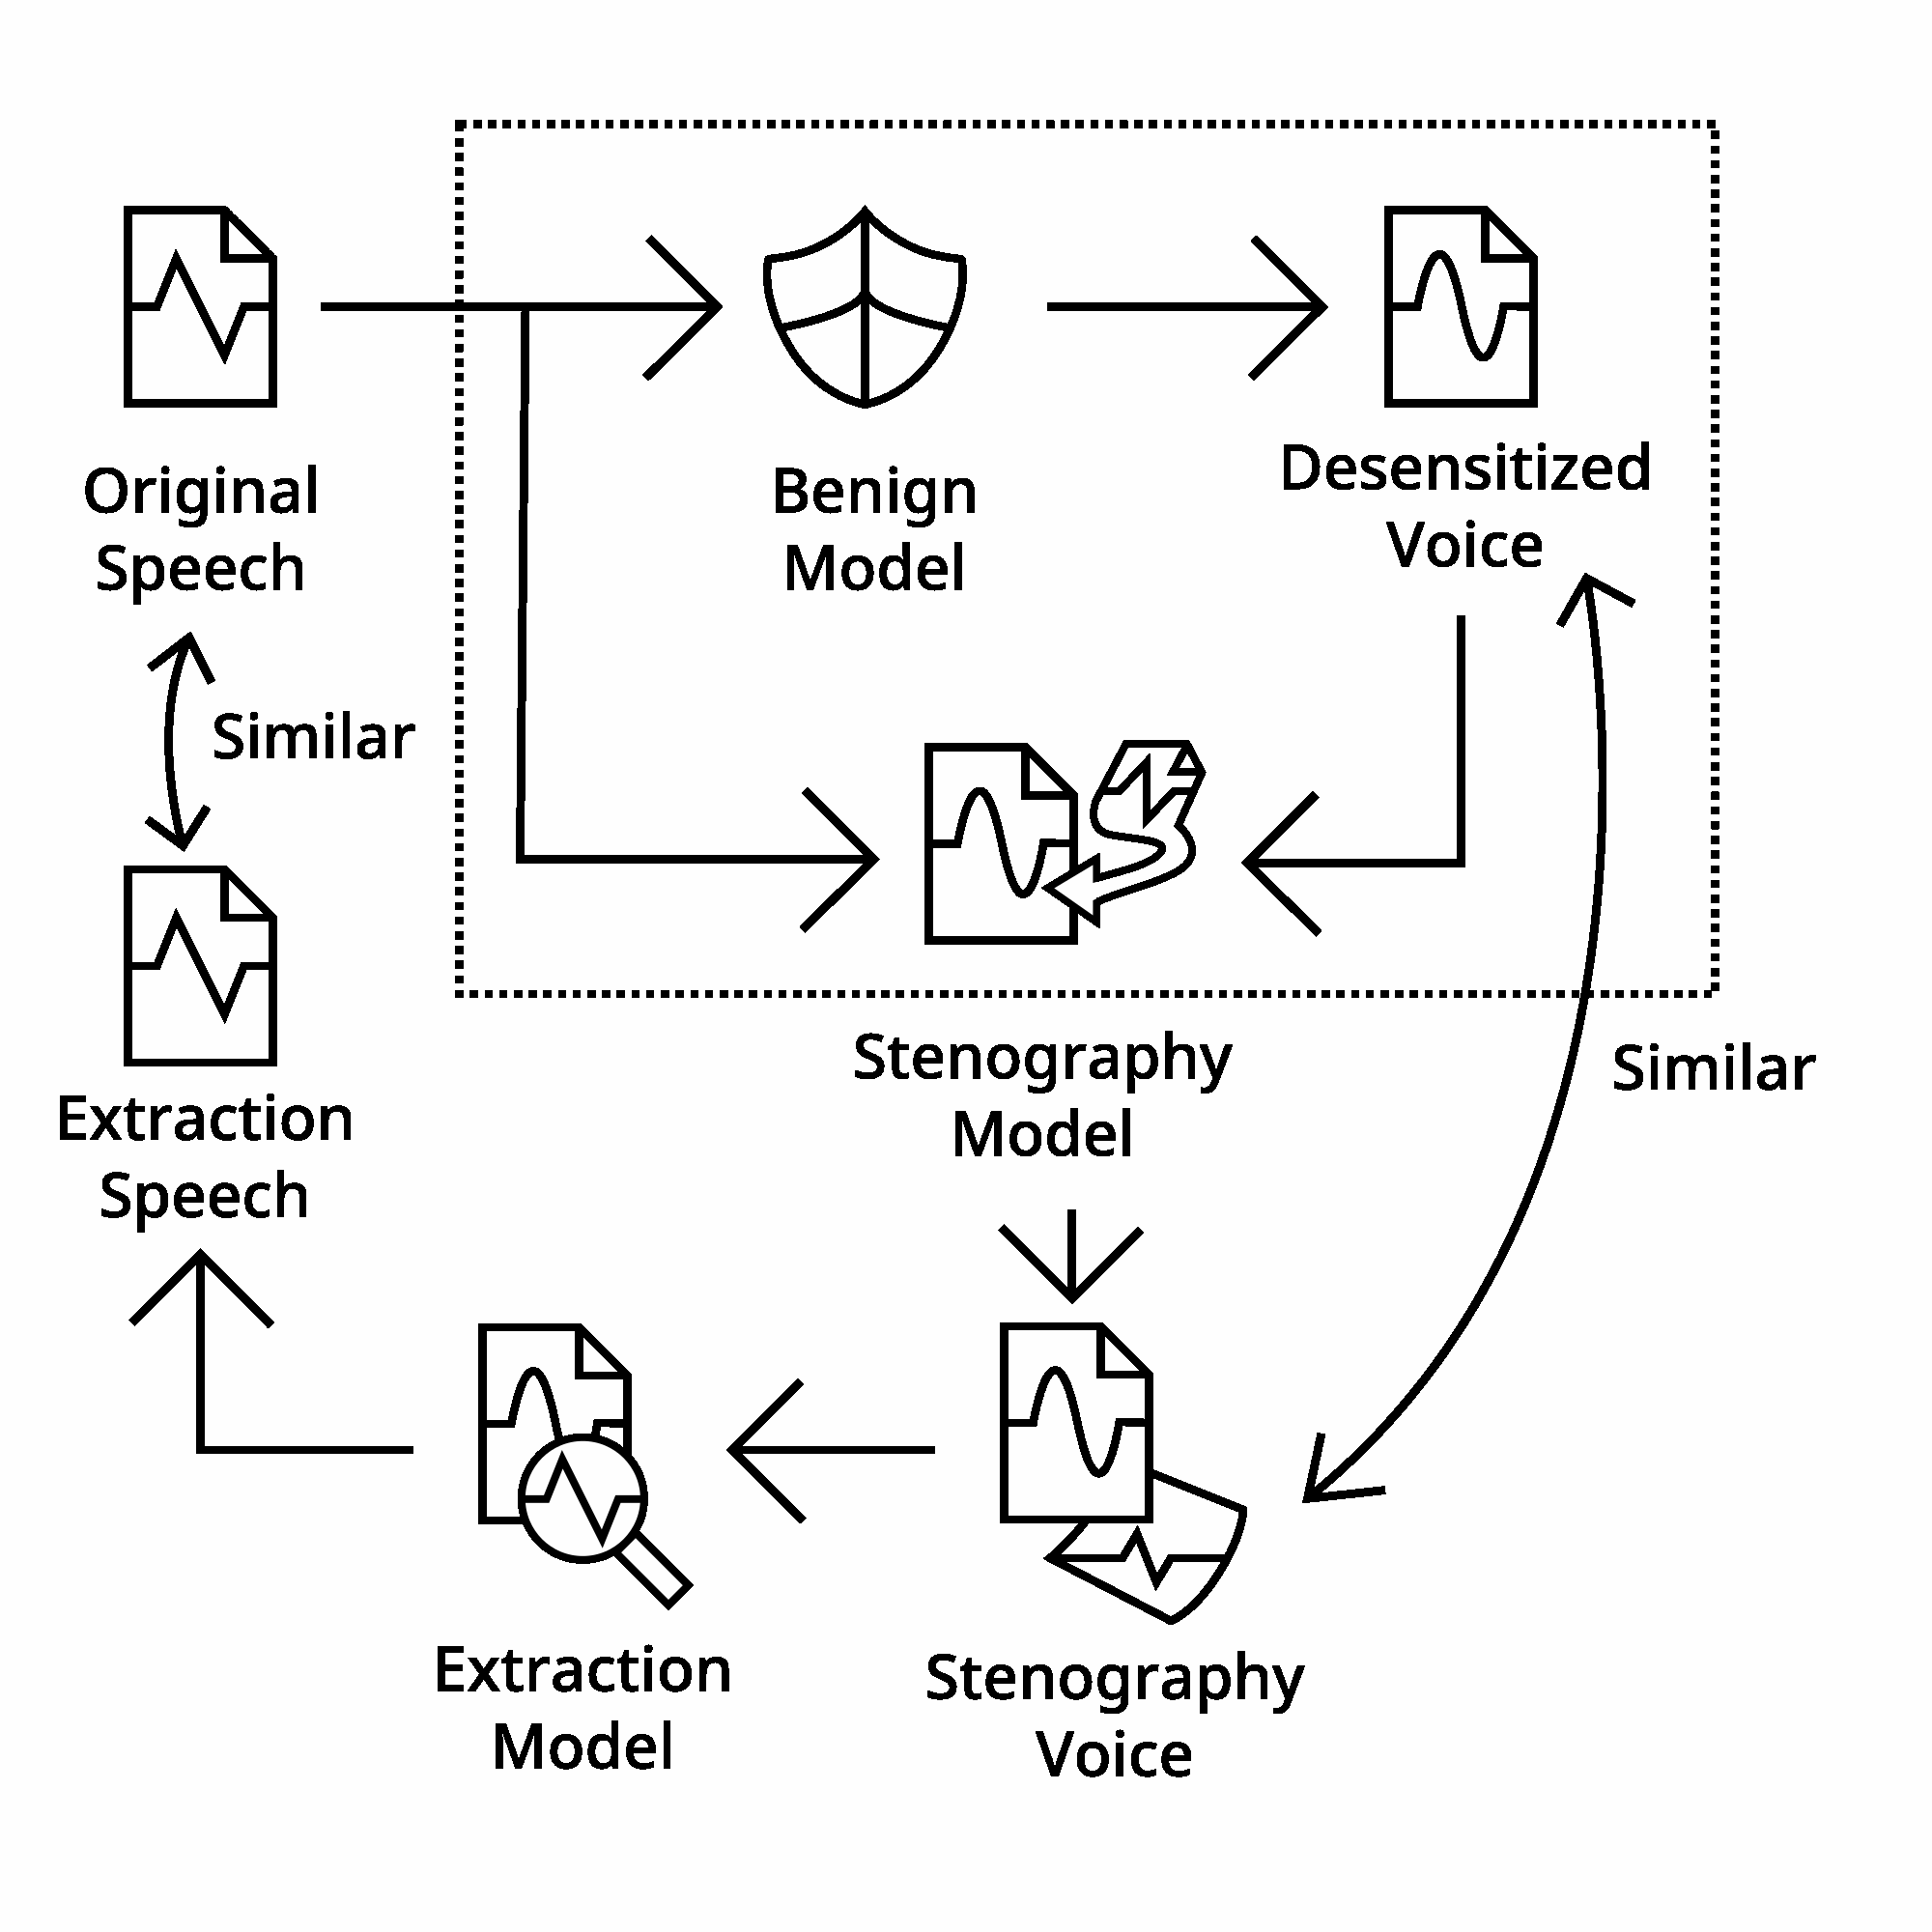
\includegraphics[width=8cm]{method.png}}
    \caption{Overview of Proposed Methodology}
    \label{overview}
\end{figure}

Our proposed adversary framework primarily works as an add-on to a benign (non-adversarial) voice desensitization model. The use case, as mentioned before, is depicted by Fig. 4, in which the user chose to use a black-box that disguised itself to be a normal desensitization service, but embedded additional data on top of the desensitized voice sequence for adversarial purposes.

And as depicted in Fig. 5, the "corrupted shield" black-box desensitization service in Fig. 4 is the workflow of our adversary. The structure we designed for the adversary closely resembles a transformer, for the reason mentioned before, that the model we are performing adversary on is conventionally a transformer model. With this particular type of structure, the nature of the desensitization model to be a black-box stay unchanged and there is no additional input or output needed, thus reduced overall suspicion.

Despite the fact that desensitization and stenography are separated steps as we presented in Fig. 5, they are in the same black-box, as the dashed-line-surrounded part in the figure. Even though we did not experiment with it, we consider it feasible to combine these two sections to form a unified adversarial desensitization model. As it's a part of the discussion topics on our proposed methodology, it will be further discussed below.

In order to complete such workflow, three distinct models are needed as depicted in Fig. 5. They are explained in detail below, but they can also be summarized as following:
\begin{itemize}
    \item A \textbf{Benign model} to be attacked by. This model generates desensitized voice sequences that users would normally want to get from this black-box.
    \item A \textbf{Stenography model} to embed features of original voice sequences on the desensitized ones. The output sequences should trick users into believing it's clean desensitized ones.
    \item A \textbf{Extraction model} to extract the features that \textbf{Stenography model} hid in the voice sequences and recover original ones from them.
\end{itemize}

\subsection{Benign model}

As two slightly different scenarios, the benign model could be either a in-house solution designed by the attacker itself (and may be even trained with adversarial models) or a production model with predefined weights acquired from a third-party organization or the public. The source of benign model theoretically shows no significant difference in terms of the overall structure of the adversary workflow we designed, but the desensitization performance of different models may have an impact on the quality of stenography-added voices and recovered ones. For our experiments we used an StarGAN-VC\cite{a3} based model, the StarGanVCDialectConversion project hosted by user "Didnelpsun" on GitHub\cite{a2} in particular.

Specifically, this specific StarGAN-VC implementation employs a transformer-based, multi-layered architecture for its generation model, which closely resemble the approach mention in the original StarGAN-VC publication. There are 5 sets of layers in both the encoder and decoder with each set of layer consisting of two convolution layers and two instance normalization layers. It's notable that this particular model is not strictly designed for desensitization, but we consider the fact that this model is capable to erase the original identity from the voice sequence and give it another one to be the ability to desensitize.

\subsection{Stenography model}

The stenography model works as an intermediate between the user and the benign model to embed information of original voice into clean product of the benign model. It's clear that, users of this adversarial product are not intended to notice the presence of such stenography model that attempts to tamper the clean output.

Details are discussed in the following sections. However, the characteristics a stenography model needed to be adequate for this purpose can be summarized as follows:

\begin{itemize}
    \item \textbf{Integration with benign model}: The stenography model should not alienate the adversary workflow by requiring additional data, other than what is provided inside the black-box (the original voice sample and the desensitized one) or be able to be detected despite being inside the black-box.
    \item \textbf{Sufficient performance}: The stenography model should embed sufficient information for the extraction model to recover the original voice sequence, thus ensuring the possibility of the adversary. But it should also avoid excess modifications applied to the samples to reduce suspicion.
\end{itemize}

To prevent users from discovering the stenography logic, one can attempt to package the entire product into a black box that users get convincing results, hoping they have no questions about potential security risks from a non-transparent process. 

However, such actions may rise suspicion among users, which may not be desired in some cases. Another robust solution to this problem is to embed the stenography model into the victim, as an additional set of layers for "post-processing", thus integrated with it. In this way, the presence of stenography model could no longer be easily detected without dedicated research of behaviour or, even, source code.

Also, the benign desensitization model attempts to replace a certain amount of features of original voices with features that does not belong to the owner of them while the stenography model attempts to embed a certain amount of information of original features into the already-desensitized voices. 

It's very likely that during this process the textual content of the voice or the overall audio quality will experience degradation to a degree. For this reason, the stenography model chosen for this purpose should be high quality enough to avoid excessively modifying the voice output.

There exist a number of solutions for this purpose\cite{a5}. In order to achieve such a task to hide sufficient information in desensitized ones while minimizing the differences made, we employed the Hide and Speak model\cite{a4}, an voice-centralized stenography model that could be considered as state of the art as it handles different lengths of carrier data and target data and produce high quality results.

\subsection{Extraction model}

The extraction model accepts the final product from the combination of benign and stenography model, which is likely to be the voices user trusted to be desensitized, and attempts recovery of original voice from it. As a model trained in conjunction with the stenography model, the one we employed in our experiment is also from the Hide and Speak mentioned before.

\section{Experiment}

\subsection{Setup}

As mentioned before, we use StarGANVCDialectConversion, a StarGAN-VC implementation as the benign model to produce desensitized voices, Hide and Speak for stenography and extraction process. All our experiments are performed on a x86-64 based container-enabled Linux server with a NVIDIA Tesla V100 GPU. We used software packages required by each models, but with Python 1.10 and PyTorch 1.13, which are slightly newer.

 For convenience of further processes, we used voice samples from TM1, TM2, SF1 and SF2, speakers in the VCC2016 data set\cite{a16}, a well-known data set that is used by numerous projects and is versatile\cite{a17, a18}, as preferred by the configuration of benign model. The voices of TM1 is considered the original voices that contain sensitive information and ones of SF1, on the other hand, is considered desensitized. With this setup in mind, the experiment can be described as: Voices of TM1 are transformed into ones of SF1 by the benign model, and the stenography model takes the output and embed voice data of TM1, generating the final output. Extraction model then use the final output to recover the voices of TM1.

\subsection{Training}

We trained the models locally on the server. In order to streamline the experiment process while preserving the most accurate possible results, we avoid excess modifications to the models. Particularly, the benign model is trained to 200000 steps (~60 epochs), as the default settings. Similar approach is applied on the stenography model, that it is trained to preferred settings by the model authors.

\subsection{Generation}

It's necessary to clarify that, in order to achieve the maximum quantity of samples and prevent the quality of benign model from having excess impact on our overall process, we use the whole VCC2016 training set as the original voices. Each identity contains 162 samples, and we get 648 samples in total.

As a StarGAN-based model, our benign model is capable to transform a voice sequence from any known speakers to another. We consider the fact that the transformed voice belongs to other identity than the original speaker to be a form of desensitization, as mentioned before. Since each sample can be used to generate 3 sequences targeting different speakers, we get 1944 in total.

The remaining steps are straightforward. We used each sample generated by benign model to get a stenography one with the original sample associated with it. Finally we used the extraction model to recover each voices.

\subsection{Evaluation}

In order to generate creditable numbers for our voice samples that correctly reflect the amount of sensitive data, the identity of original speaker, we employed cloud-based voiceprint analysis solution provided by iFlyTek. After learning about the identity of four speakers in our domain, this service is able to generate 4 numbers for each voice sample, denoting the probability of the voice to belong to a particular speaker. iFlyTek suggests in the official manual that a score that is higher than 0.6 meant that the identity of a sample can be confirmed. We consider the identity with the highest score for a particular sample to be the classification made by this service.

\section{Results}

\subsection{Explanation}

Table I to IV presents the essential statistics of our results. All of the statistics are based on the score of each sample being classified into the original identity of their own. A higher score mean that our evaluation service, as mentioned before, deduces that the sample has a higher probability to belong to its original identity.

Each row contains statistics targeting the original identity of samples where their original identity is the speaker denoted in the header. Each column consists different types of results of statistical computation according to the following description:

\begin{itemize}
    \item \textbf{Mean} - Average value of scores. Higher values mean generally closer to the original speaker.
    \item \textbf{Definiteness} - Ratio of scores being greater than 0.6, which means the sample can be confirmed to bear the same speaker as the original one. Higher values mean values are more definite.
    \item \textbf{Best} - Best value of scores.
    \item \textbf{Worst} - Worst value of scores. Closer value with \textbf{Best} means better stability.
    \item \textbf{Class Ratio} - Ratio of samples being classified into its original speaker, i.e. have the highest score being the original speaker, as mentioned before. Higher values mean higher probability an generic classification model will think the samples have the same identity of the original speakers.
\end{itemize}

\subsection{Analysis}

\subsubsection{Original samples}

According to Table I, all of the score statistics, except for the \textbf{Worst}, are close to 1, which is intended behavior for original samples. As the worst case, \textbf{Worst} is also close or greater than 0.6, which means that even this type of cases are confirmed to have the same identity as the original speaker. As a result, it's safe to confirm that both the benign model and the validation service are of desirable performance.

\subsubsection{Desensitized samples}

According to Table II, the overall score dropped drastically from over 0.8 to over 0.4. It can be argued that from the \textbf{Best} and \textbf{Class Ratio} numbers that there still exhibits a portion of samples that are classified into the original speaker. However, these type of classification results can not be trusted because they are vague, according to the close-to-zero \textbf{Definiteness} value.

\subsubsection{Stenography samples}

Scores of stenography samples are similar to the desensitized ones, given the numerical changes of statistical numbers are mostly less than 0.1. However, the changes stenography model made to the samples did not cause any form of degradation of desensitization performance, but upgraded it instead.

Table V is the statistics of direct comparison between these two sets of samples. According to the \textbf{Minimum} value, it's still possible that the desensitization performance would suffer significant degradation from the stenography process, but from the \textbf{Mean} and \textbf{Variance} value we can see that the performance changes are even-spread.

It's highly likely that the changes are caused by the slight content degradation, i.e. perturbation, made by stenography model and would not strongly affect the overall performance of such adversary. We also performed manual audio quality tests on a random subset of this set of samples and confirmed that the degradation is not audible.

\subsubsection{Extracted samples}

As mentioned before, extracted samples are meant to be as close to the original samples as possible. As presented in Table IV, the values are slightly inferior than the original samples with the decrease of score within 0.1 to 0.2. However, despite the worsen results, the \textbf{Definiteness} and \textbf{Class Ratio} are still well desirable, suggesting that the usability of these samples are comparable to the original ones, which declares the success of adversary.

\begin{table}[htbp]
    \centering
    \caption{Statistics of Original Samples}
    \begin{tabular}{|c|c|c|c|c|}
        \hline
        & \textbf{SF1} & \textbf{SF2} & \textbf{TM1} & \textbf{TM2} \\
        \hline
        \textbf{Mean} & 0.853889 & 0.837284 & 0.84537 & 0.837963 \\
        \hline
        \textbf{Definiteness} & 1.0 & 0.987654 & 1.0 & 1.0 \\
        \hline
        \textbf{Best} & 0.95 & 0.94 & 0.94 & 0.94 \\
        \hline
        \textbf{Worst} & 0.6 & 0.56 & 0.6 & 0.61 \\
        \hline
        \textbf{Class Ratio} & 1.0 & 1.0 & 1.0 & 1.0 \\
        \hline
    \end{tabular}
    \label{tab:st_org}
\end{table}

\begin{table}[htbp]
    \centering
    \caption{Statistics of Desensitized Samples}
    \begin{tabular}{|c|c|c|c|c|}
        \hline
        & \textbf{SF1} & \textbf{SF2} & \textbf{TM1} & \textbf{TM2} \\
        \hline
        \textbf{Mean} & 0.407654 & 0.440206 & 0.460556 & 0.417078 \\
        \hline
        \textbf{Definiteness} & 0 & 0.022634 & 0.047325 & 0.004115 \\
        \hline
        \textbf{Best} & 0.58 & 0.64 & 0.62 & 0.62 \\
        \hline
        \textbf{Worst} & 0.22 & 0.23 & 0.27 & 0.21 \\
        \hline
        \textbf{Class Ratio} & 0.125514 & 0.236626 & 0.195473 & 0.012346 \\
        \hline
    \end{tabular}
    \label{tab:st_des}
\end{table}

\begin{table}[htbp]
    \centering
    \caption{Statistics of Stenography Samples}
    \begin{tabular}{|c|c|c|c|c|}
        \hline
        & \textbf{SF1} & \textbf{SF2} & \textbf{TM1} & \textbf{TM2} \\
        \hline
        \textbf{Mean} & 0.387695 & 0.366070 & 0.412119 & 0.394115 \\
        \hline
        \textbf{Definiteness} & 0 & 0.002058 & 0 & 0 \\
        \hline
        \textbf{Best} & 0.52 & 0.61 & 0.56 & 0.56 \\
        \hline
        \textbf{Worst} & 0.21 & 0.15 & 0.17 & 0.20 \\
        \hline
        \textbf{Class Ratio} & 0.119342 & 0.183128 & 0.1893 & 0.014403 \\
        \hline
    \end{tabular}
    \label{tab:st_msg}
\end{table}

\begin{table}[htbp]
    \centering
    \caption{Statistics of Extracted Samples}
    \begin{tabular}{|c|c|c|c|c|}
        \hline
        & \textbf{SF1} & \textbf{SF2} & \textbf{TM1} & \textbf{TM2} \\
        \hline
        \textbf{Mean} & 0.681975 & 0.681728 & 0.695123 & 0.702593 \\
        \hline
        \textbf{Definiteness} & 0.901235 & 0.864198 & 0.950617 & 0.938272 \\
        \hline
        \textbf{Best} & 0.81 & 0.81 & 0.81 & 0.85 \\
        \hline
        \textbf{Worst} & 0.44 & 0.47 & 0.53 & 0.46 \\
        \hline
        \textbf{Class Ratio} & 0.993827 & 1 & 1 & 0.993827 \\
        \hline
    \end{tabular}
    \label{tab:st_rec}
\end{table}

\begin{table}[htbp]
    \centering
    \caption{Statistics of Differences Between Desensitized and Stenography Samples}
    \begin{tabular}{|c|c|}
        \hline
        \textbf{Mean} & 0.041373 \\
        \hline
        \textbf{Variance} & 0.010478 \\
        \hline
        \textbf{Maximum} & 0.37 \\
        \hline
        \textbf{Minimum} & -0.29 \\
        \hline
        \textbf{Maximum Absolute Value} & 0.37 \\
        \hline
        \textbf{Minimum Absolute Value} & 0 \\
        \hline
    \end{tabular}
\end{table}

\section{Discussion}

According to our experiments, it is safe to consider conventional acoustical-based or NN-based audio transforming solutions not sufficient for voice desensitization. Besides the StarGAN-VC solution we used, there exists many more such "voice changer" services on the Internet available for public use. One would consider these solutions secure because of the vast audible differences they made on its voice sequences. However, these solution exhibits potential of adversary with such method we demonstrated in this paper, which is not negligible. It's not likely that human ears can pick up subtle changes a stenography program made to certain parts of a voice sequence.

It's possible to avoid or mitigate risks of being attacked by such method. The most straightforward way to go is to avoid desensitization models from unknown or unsound sources. Due to the black-box nature of various proprietary services, it is not likely possible for users to have practical means to test these services for potential adversaries. When possible, users could train their own desensitization models. If the models are acquired from third-party, users should pay attention to the behaviour of model and the choice of training data set.

\section{Future Work}

In our experiment, we simply directed the voice sequence generated by the benign model to the stenography model. As mentioned before, this approach may not be sufficient in terms of stealthiness. Also, the overall storage consumption of this black box will increase significantly and the processing performance may not be ideal. 

We believed that turning the stenography model into extra layers of benign model, eliminating the redundant audio encoding and decoding processes, can mitigate such problems while potentially increase the overall adversarial quality. In this way, the benign model can train in conjunction with the adversary model, taking advantage of intermediate representations of it. Moreover, this creates the potential of reducing the overall storage consumption and be less suspicious.

As another way to mitigate such problem, users can use various traditional or ML-based methods to apply inaudible perturbation on processed voices to attempt erasure of potential stenography while preserving high audio quality.

\section{Conclusion}

Targeting voice desensitization models based on generative NN models, we designed an adversary scheme that attempts to recover original voices from desensitized ones via stenography means, thus cause a privacy bleach. Our experiments prove this idea to be viable and the conventional solutions to be vulnerable to this type of adversary.

\begin{thebibliography}{00}
    \bibitem{a1} N. Subramanian, O. Elharrouss, S. Al-Maadeed and A. Bouridane, "Image Steganography: A Review of the Recent Advances," in IEEE Access, vol. 9, pp. 23409-23423, 2021, doi: 10.1109/ACCESS.2021.3053998.
    \bibitem{a2} https://github.com/Didnelpsun/StarGanVCDialectConversion
    \bibitem{a3} Y. Li, X. Qiu, P. Cao, Y. Zhang, and B. Bao, “Non-parallel Voice Conversion Based on Perceptual Star Generative Adversarial Network,” Circuits Syst Signal Process, vol. 41, no. 8, pp. 4632–4648, Aug. 2022, doi: 10.1007/s00034-022-01998-5.
    \bibitem{a4} F. Kreuk, Y. Adi, B. Raj, R. Singh, and J. Keshet, “Hide and Speak: Towards Deep Neural Networks for Speech Steganography.” arXiv, Jul. 27, 2020. doi: 10.48550/arXiv.1902.03083.
    \bibitem{a5} N. Takahashi, M. K. Singh, and Y. Mitsufuji, “Source Mixing and Separation Robust Audio Steganography.” arXiv, Feb. 17, 2022. doi: 10.48550/arXiv.2110.05054.
    \bibitem{a6} Andreas Nautsch, Abelino Jiménez, Amos Treiber, Jascha Kolberg, Catherine Jasserand, Els Kindt, Héctor Delgado, Massimiliano Todisco, Mohamed Amine Hmani, Aymen Mtibaa, Mohammed Ahmed Abdelraheem, Alberto Abad, Francisco Teixeira, Driss Matrouf, Marta Gomez-Barrero, Dijana Petrovska-Delacrétaz, Gérard Chollet, Nicholas Evans, Thomas Schneider, Jean-François Bonastre, Bhiksha Raj, Isabel Trancoso, and Christoph Busch. 2019. Preserving privacy in speaker and speech characterisation. Comput. Speech Lang. 58, C (Nov 2019), 441–480. https://doi.org/10.1016/j.csl.2019.06.001
    \bibitem{a7} Kröger, J.L., Lutz, O.HM., Raschke, P. (2020). Privacy Implications of Voice and Speech Analysis – Information Disclosure by Inference. In: Friedewald, M., Önen, M., Lievens, E., Krenn, S., Fricker, S. (eds) Privacy and Identity Management. Data for Better Living: AI and Privacy. Privacy and Identity 2019. IFIP Advances in Information and Communication Technology(), vol 576. Springer, Cham.
    \bibitem{a8} Jaemin Lim, Kiyeon Kim, Hyunwoo Yu, and Suk-Bok Lee. 2022. Overo: Sharing Private Audio Recordings. In Proceedings of the 2022 ACM SIGSAC Conference on Computer and Communications Security (CCS '22). Association for Computing Machinery, New York, NY, USA, 1933–1946. https://doi.org/10.1145/3548606.3560572
    \bibitem{a9} J. Qian, H. Du, J. Hou, L. Chen, T. Jung and X. -Y. Li, "Speech Sanitizer: Speech Content Desensitization and Voice Anonymization," in IEEE Transactions on Dependable and Secure Computing, vol. 18, no. 6, pp. 2631-2642, 1 Nov.-Dec. 2021, doi: 10.1109/TDSC.2019.2960239.
    \bibitem{a10} Jianwei Qian, Haohua Du, Jiahui Hou, Linlin Chen, Taeho Jung, and Xiang-Yang Li. 2018. Hidebehind: Enjoy Voice Input with Voiceprint Unclonability and Anonymity. In Proceedings of the 16th ACM Conference on Embedded Networked Sensor Systems (SenSys '18). Association for Computing Machinery, New York, NY, USA, 82–94. https://doi.org/10.1145/3274783.3274855
    \bibitem{a11} J. Qian, F. Han, J. Hou, C. Zhang, Y. Wang and X. -Y. Li, "Towards Privacy-Preserving Speech Data Publishing," IEEE INFOCOM 2018 - IEEE Conference on Computer Communications, Honolulu, HI, USA, 2018, pp. 1079-1087, doi: 10.1109/INFOCOM.2018.8486250.
    \bibitem{a12} Nandwana, Mahesh Kumar, Julien van Hout, Mitchell McLaren, Allen R. Stauffer, Colleen Richey, Aaron D. Lawson and Martin Graciarena. “Robust Speaker Recognition from Distant Speech under Real Reverberant Environments Using Speaker Embeddings.” Interspeech (2018).
    \bibitem{a13} https://docs.aws.amazon.com/transcribe/latest/dg/pii-redaction.html
    \bibitem{a14} Vidizmo - Automatic audio redaction software. https://www.vidizmo/com/vidizmo-artificial-intelligence-solutions/redaction/
    \bibitem{a15} Audacity - Open source audio software. https://www.audacityteam.org/
    \bibitem{a16} T. Toda, L.-H. Chen, D. Saito, F. Villavicencio, M. Wester, Z. Wu, J. Yamagishi, "The Voice Conversion Challenge 2016," Proc. INTERSPEECH, pp. 1632-1636, 2016.
    \bibitem{a17} M. Wester, Z. Wu, J. Yamagishi, "Analysis of the Voice Conversion Challenge 2016 Evaluation Results," Proc. INTERSPEECH, pp. 1637-1641, 2016.
    \bibitem{a18} M. Wester, Z. Wu, J. Yamagishi, "Multidimensional scaling of systems in the Voice Conversion Challenge 2016," Proc. SSW9, pp. 40-45, 2016.
    \bibitem{a19} Siri - Voice assistant software. https://www.apple.com/siri/
    \bibitem{a20} Xiao Ai - Voice assistant software. https://xiaoai.mi.com/
    \bibitem{a21} iFly Input Method - Chinese/English input method software. https://srf.xunfei.cn
    \bibitem{a22} GBoard - Multilingual input method software. https://play.google.com/store/apps/details?id=com.google.android.inputmethod
\end{thebibliography}

\end{document}
